\section{Analisi}
Inizialmente sono state condotte una serie di analisi con l'obiettivo principale di individuare il modello più promettente. Successivamente, ci si è dedicati all'indagine delle configurazioni più adatte del momento, al fine di massimizzare l'accuratezza del sistema.

\subsection{Scelta del Modello}
Per identificare il modello ottimale, sono stati eseguiti diversi approfondimenti. Nel primo esperimento è stata impiegata una rete nota come \textbf{AlexNet}; successivamente è stata considerata una rete basata su essa, denominata \textbf{MiniAlexNet}; infine, introducendo sia layer di Dropout sia layer di Batch Normalization, è stata ottenuta la versione \textbf{MiniAlexNetV2}.

\begin{figure}[htbp]
\centering
\begin{minipage}[t]{0.33\textwidth}
    \centering
    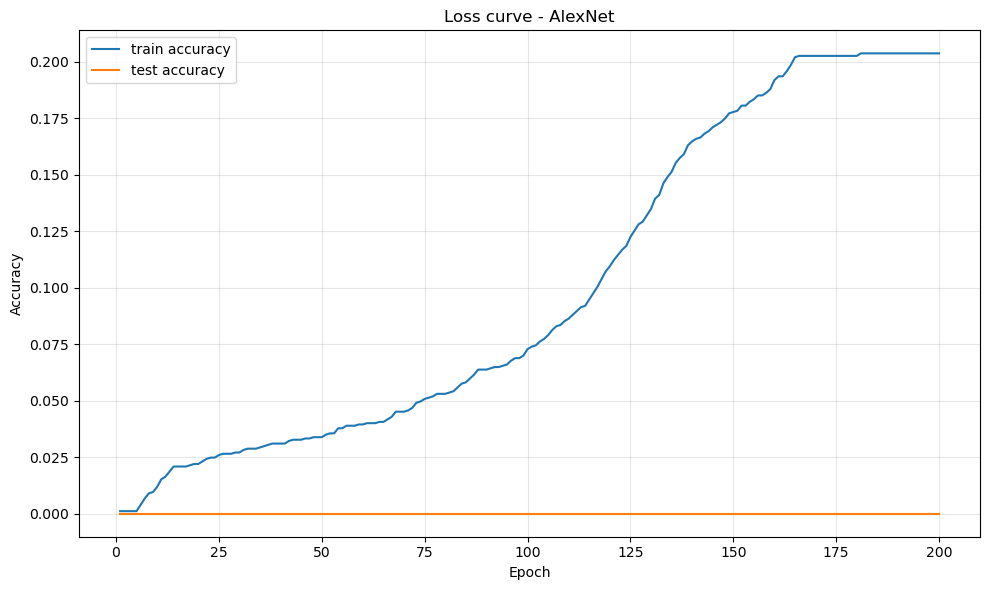
\includegraphics[width=\linewidth]{Analisi/LeNetColor_Acc.png}
\end{minipage}\hfill
\begin{minipage}[t]{0.34\textwidth}
    \centering
    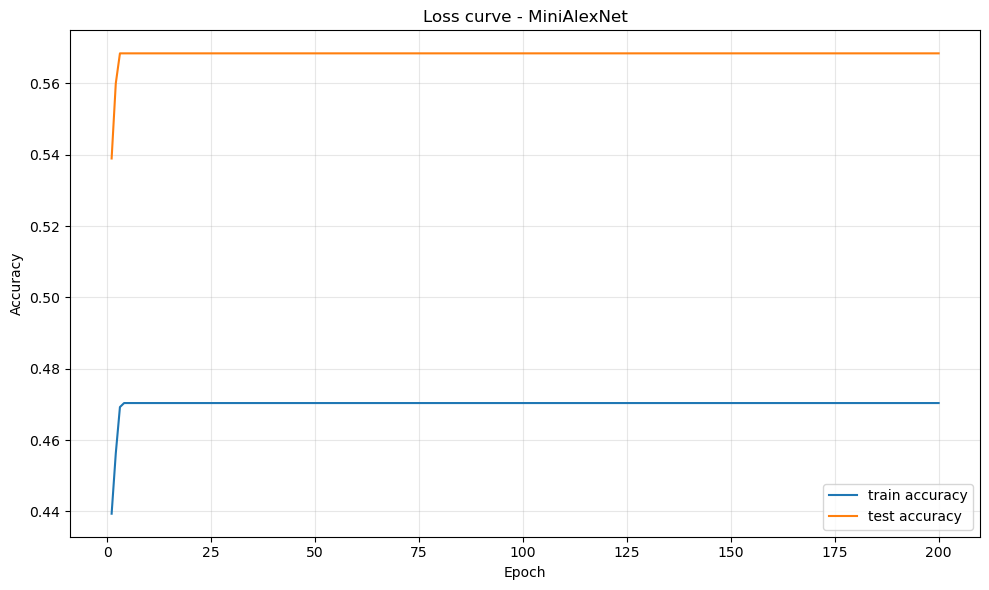
\includegraphics[width=\linewidth]{Analisi/MiniAlexNet_Acc.png}
\end{minipage}\hfill
\begin{minipage}[t]{0.33\textwidth}
    \centering
    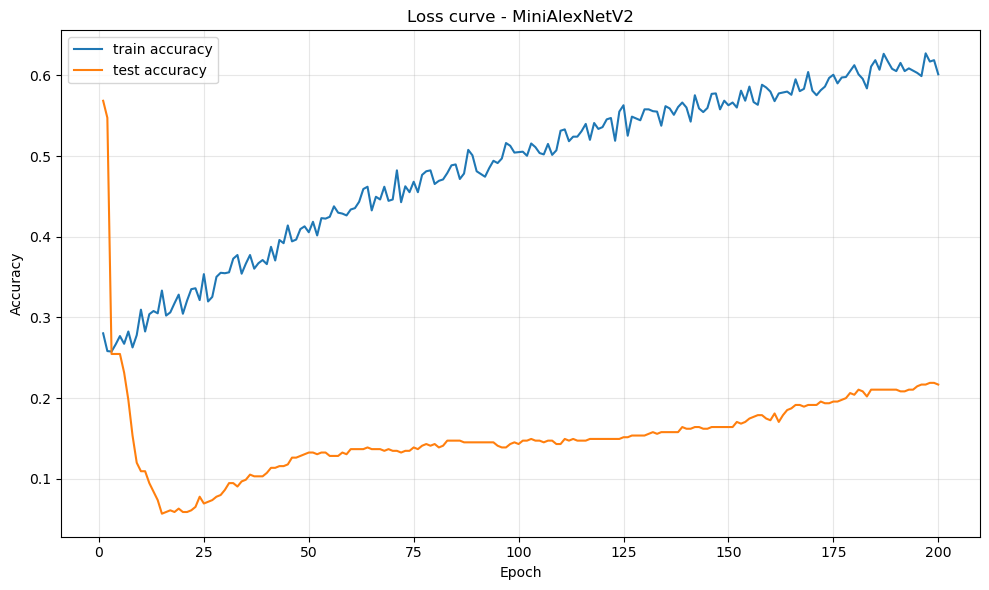
\includegraphics[width=\linewidth]{Analisi/MiniAlexNetV2_Acc.png}
\end{minipage}

\caption{Confronto tra le curve di accuratezza delle tre reti}
\label{fig:Acc}
\end{figure}

L'esame della Figura \ref{fig:Acc} evidenzia in modo chiaro come la rete \textbf{MiniAlexNetV2} raggiunga un'accuratezza sensibilmente superiore rispetto alle altre due configurazioni. In particolare, la \textbf{MiniAlexNet} mostra un andamento poco stabile e complessivamente modesto, mentre la rete \textbf{AlexNet} presenta un comportamento migliore rispetto alla MiniAlexNet, pur rimanendo inferiore alla MiniAlexNetV2. Pertanto, dal punto di vista dell'accuratezza, la rete MiniAlexNetV2 emerge come la soluzione più efficace.

\begin{figure}[htbp]
\centering
\begin{minipage}[t]{0.33\textwidth}
    \centering
    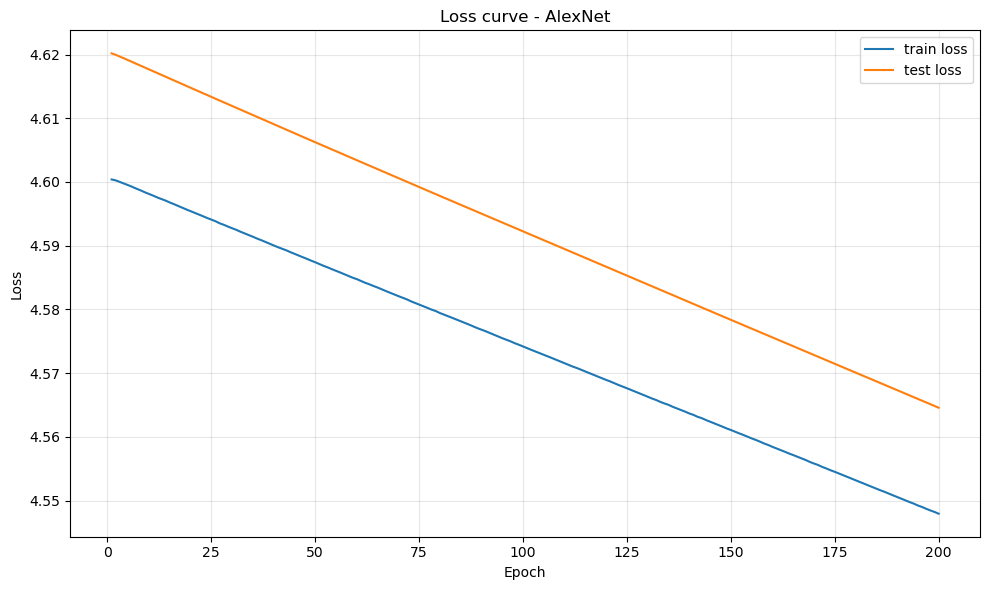
\includegraphics[width=\linewidth]{Analisi/LeNetColor_Loss.png}
\end{minipage}\hfill
\begin{minipage}[t]{0.34\textwidth}
    \centering
    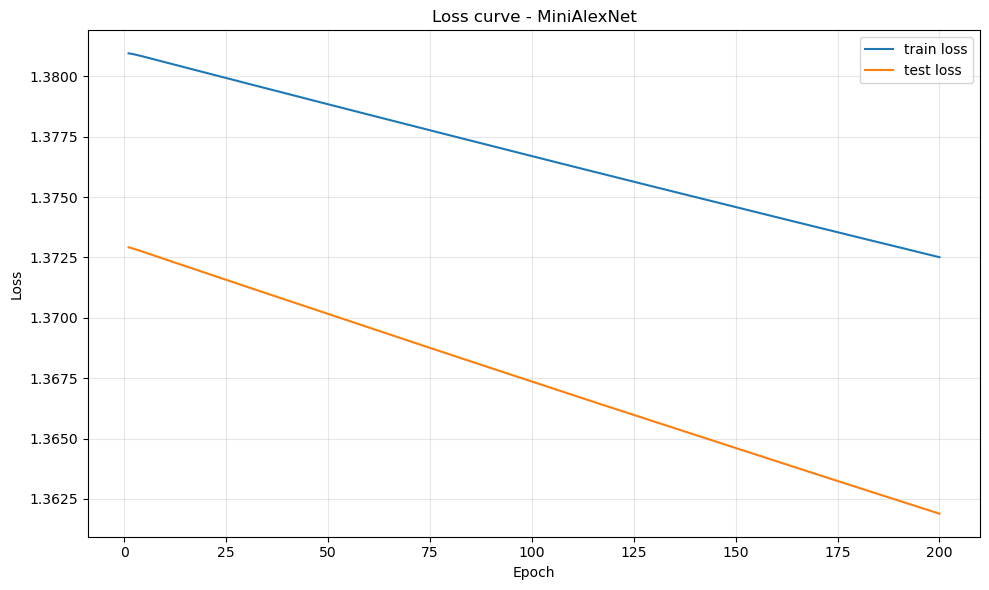
\includegraphics[width=\linewidth]{Analisi/MiniAlexNet_Loss.png}
\end{minipage}\hfill
\begin{minipage}[t]{0.33\textwidth}
    \centering
    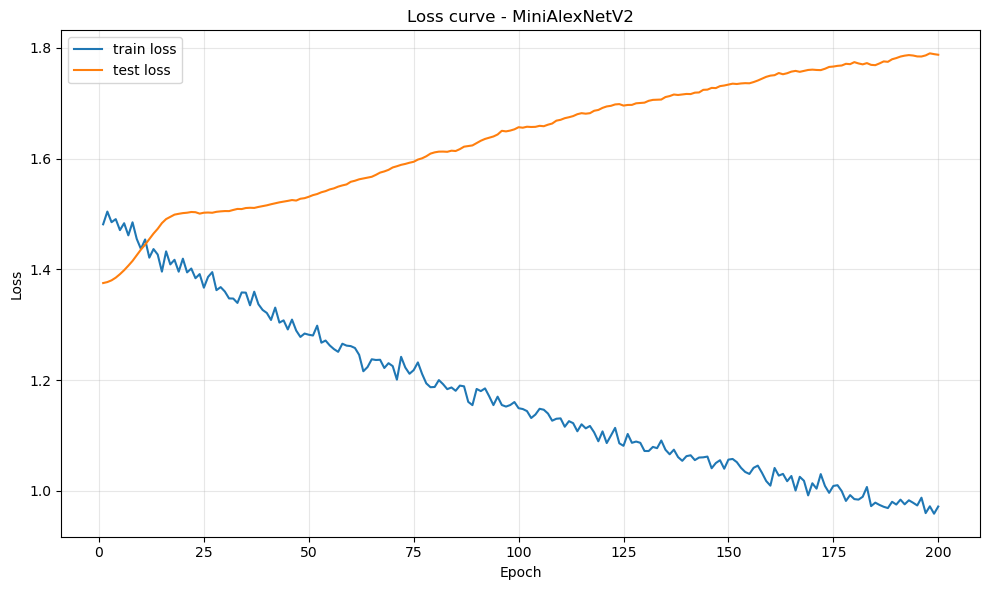
\includegraphics[width=\linewidth]{Analisi/MiniAlexNetV2_Loss.png}
\end{minipage}

\caption{Confronto tra le curve di loss delle tre reti}
\label{fig:Loss}
\end{figure}

Dall'analisi della Figura \ref{fig:Loss} emergono differenze significative tra le tre reti, tutte addestrate per 200 epoche. La rete \textbf{MiniAlexNetV2} mostra valori di loss più bassi rispetto alle altre architetture e una dinamica di apprendimento più efficace. Tuttavia, durante la fase di test, la curva evidenzia un iniziale aumento della loss, fenomeno compatibile con una fase di instabilità nelle prime epoche di addestramento; successivamente, la curva tende a stabilizzarsi su valori più contenuti.

La rete \textbf{MiniAlexNet}, pur presentando un comportamento più regolare rispetto ad AlexNet, mostra comunque prestazioni limitate e una capacità di generalizzazione contenuta. La rete \textbf{AlexNet}, infine, evidenzia un miglioramento lieve ma complessivamente inferiore rispetto alla MiniAlexNetV2.

Nel complesso, questi risultati hanno portato a concentrare gli sforzi sull'ulteriore sviluppo della rete \textbf{MiniAlexNetV2}.

I parametri utilizzati per queste prove sono stati:
\begin{itemize}
  \item Tasso di apprendimento (\textit{Learning Rate}): 0.0001
  \item Momento (\textit{Momentum}): 0.6
\end{itemize}

\subsection{ROC Curve}
Una volta individuate le tre configurazioni più significative, il processo di training è stato reiterato per ulteriori 200 epoche e successivamente sono state calcolate le rispettive ROC curve, riportate in Figura \ref{fig:Roc}. La curva ROC, che descrive la relazione tra il tasso di veri positivi (TPR) e il tasso di falsi positivi (FPR) al variare della soglia di classificazione, è stata utilizzata come ulteriore criterio di valutazione per confrontare le capacità discriminanti dei tre modelli.

\begin{figure}[htbp]
\centering
\begin{minipage}[t]{0.33\textwidth}
    \centering
    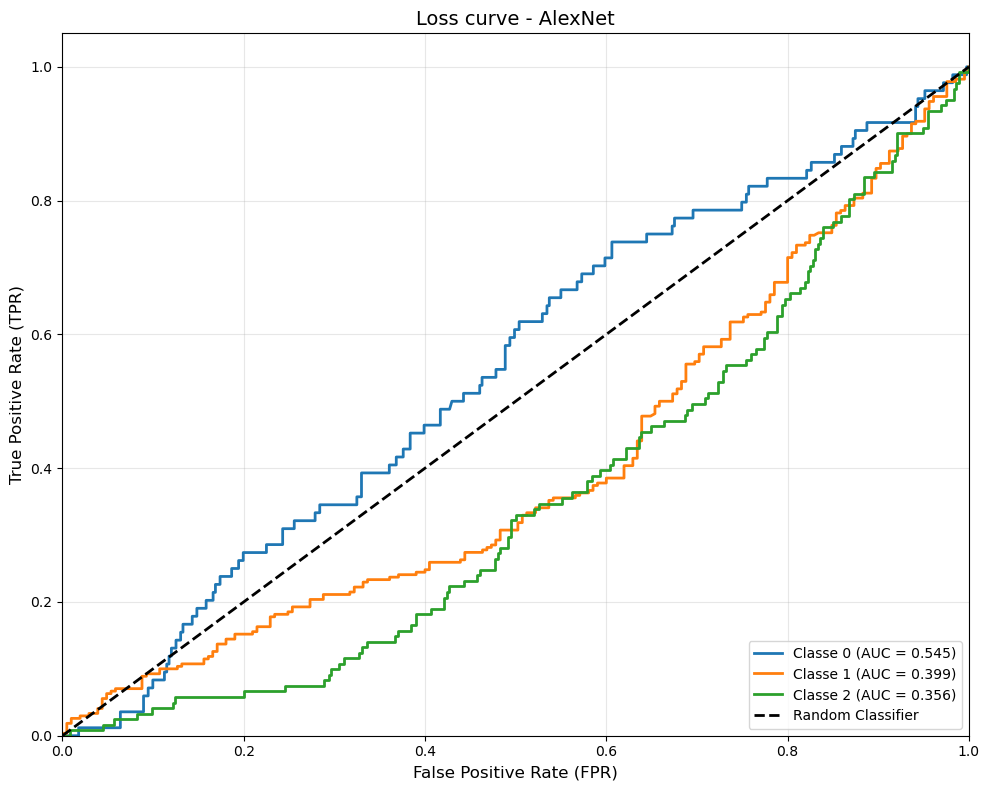
\includegraphics[width=\linewidth]{Analisi/LeNetColor_ROC.png}
\end{minipage}\hfill
\begin{minipage}[t]{0.34\textwidth}
    \centering
    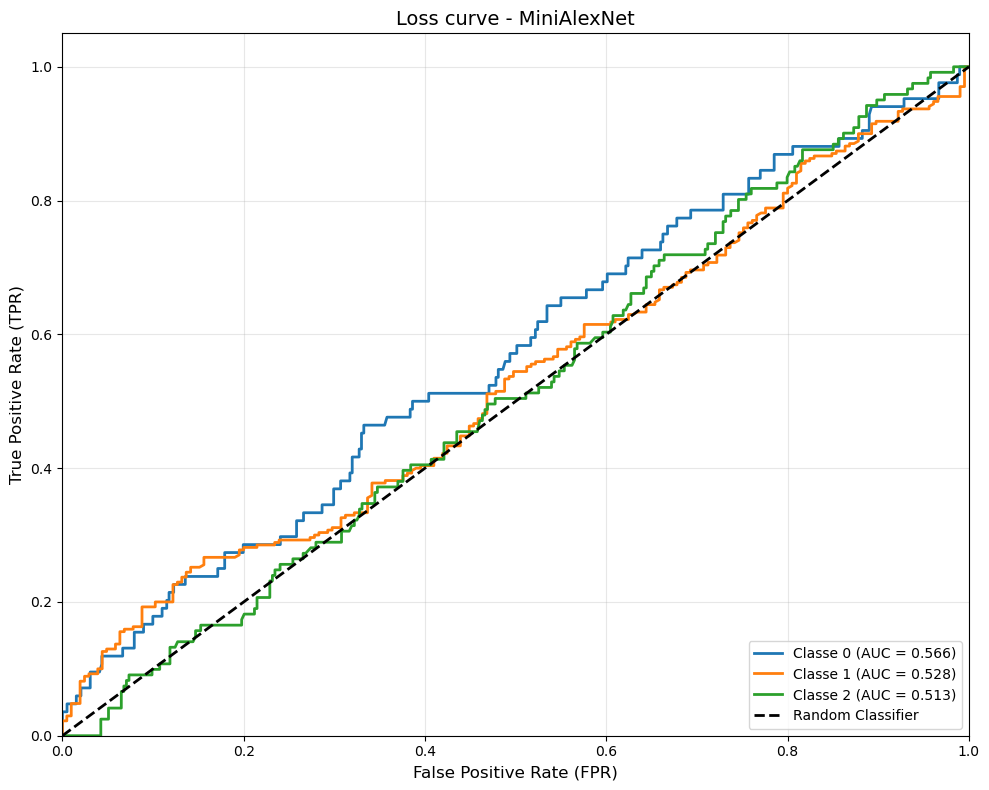
\includegraphics[width=\linewidth]{Analisi/MiniAlexNet_ROC.png}
\end{minipage}\hfill
\begin{minipage}[t]{0.33\textwidth}
    \centering
    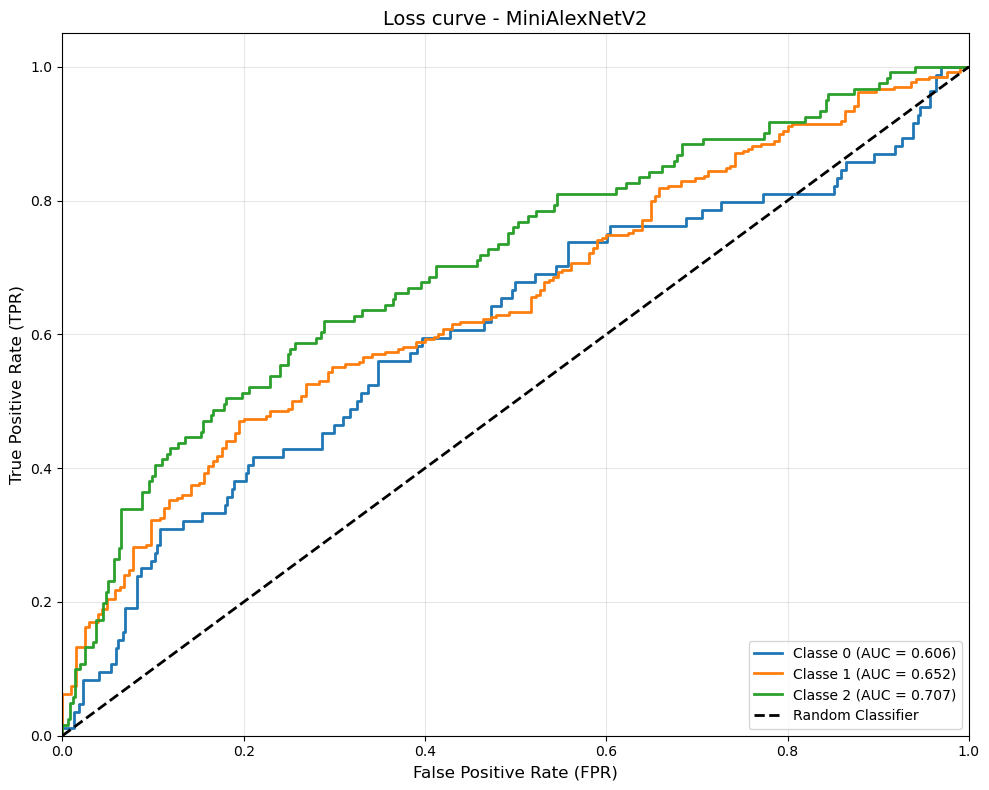
\includegraphics[width=\linewidth]{Analisi/MiniAlexNetV2_ROC.png}
\end{minipage}

\caption{Confronto tra le ROC curve delle tre reti}
\label{fig:Roc}
\end{figure}

Dall'analisi delle curve ROC in Figura \ref{fig:Roc} risulta evidente che la rete \textbf{MiniAlexNetV2} è quella con le prestazioni migliori. In particolare, i valori di AUC ottenuti sono pari a 0.606 per la classe 0, 0.652 per la classe 1 e 0.707 per la classe 2, evidenziando una capacità discriminante superiore rispetto alle altre reti. La rete \textbf{MiniAlexNet} presenta invece risultati prossimi al caso casuale, con AUC pari a 0.566, 0.528 e 0.513 rispettivamente per le tre classi. La rete \textbf{AlexNet} mostra infine le prestazioni peggiori, con AUC pari a 0.545 per la classe 0, 0.399 per la classe 1 e 0.356 per la classe 2.

Sulla base del confronto tra le tre curve ROC, la rete \textbf{MiniAlexNetV2} è stata quindi selezionata come modello più promettente, in quanto mostra il miglior compromesso tra capacità discriminante e stabilità delle prestazioni.